\begin{myposter}{
    Глава 2. Решение задачи теории удара. \\ Начальные условия для расчетов.
}

    \headerbox
    {Глава 2. Решение задачи теории удара.}
    {name=first,column=0,row=0,span=3}
    {
        {\huge\bf
            \vspace{10pt}
            \hspace{15pt}
            \minipage{0.35\textwidth}
                $$ \eqnuposleproj $$
                
                Действительно, т.к.
                $$ \mke\deltadq = \Q, \enspace \Q^T\delta\qposle = 0,$$
                $$ \dqposle = \dqdo -\ \deltadq = \mathbf{V}\nuposle \in \subspace,$$
                то
                $$ 0 = \dotp{\mke\deltadq}{\cstr} $$
                $$ = \dotp{\mke\left(\cstr\nuposle - \dqdo\right)}{\cstr} \\ $$
                $$ = \dotp{\mke\cstr\nuposle - \mke\dqdo}{\cstr} \\ $$
                $$ = \cstr^T\mke\cstr\nuposle - \cstr^T\mke\dqdo, \enspace \text{ч.т.д.} $$
            \endminipage
            \hspace{55pt}
            \minipage{0.65\textwidth}
                \begin{figure}[H]
                    \centering
                    \hspace{-92pt}
                    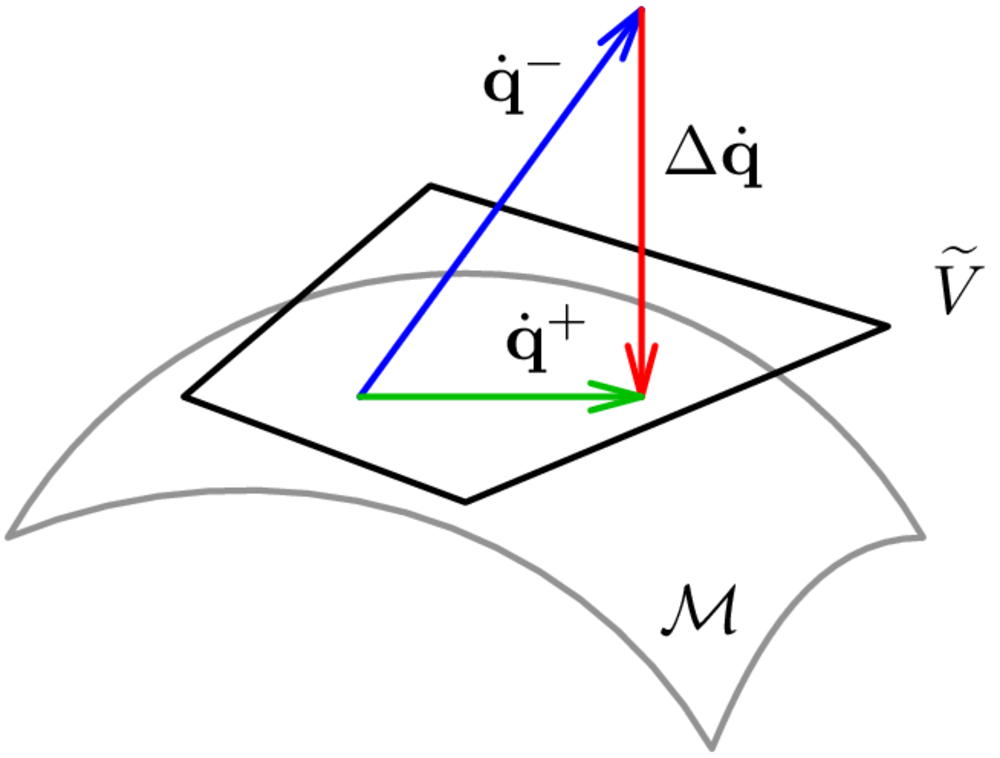
\includegraphics[width=0.8\textwidth]{content/pic/asypng/pic_project.png}
                    % \asyinclude{content/pic/asy/pic_project}
                    \qquad
                    \caption{{\huge
                        $\dqposle$ -- проекция $\dqdo$ на $\subspace$,\newline
                        ортогональная в метрике $\mke$
                    }}
                \end{figure}
            \endminipage
            \vspace{10pt}
        }
    }
    
    \headerbox
    {Начальные условия для расчетов.}
    {name=second,column=0,row=1,below=first,span=3}
    {
        {\huge\bf
            \vspace{10pt}
            \begin{itemize}
                \item отношение радиуса колеса к радиусу платформы $\ddfrac{r}{R} = \ddfrac{1}{3}$,
                \item отношение массы колеса к массе платформы $\ddfrac{M_{\text{к}}}{M_{\text{пл}}} = 0.15$, 
                \item отношение массы ролика к массе платформы $\ddfrac{m_{\text{рол}}}{M_{\text{пл}}} = 0.05$, 
                \item $\vec{\omega}_0 = 1$, $\vec{v}_0 = 1$
            \end{itemize}
            \centering
            \begin{figure}[H]
                \minipage{0.3\textwidth}
                    \centering
                    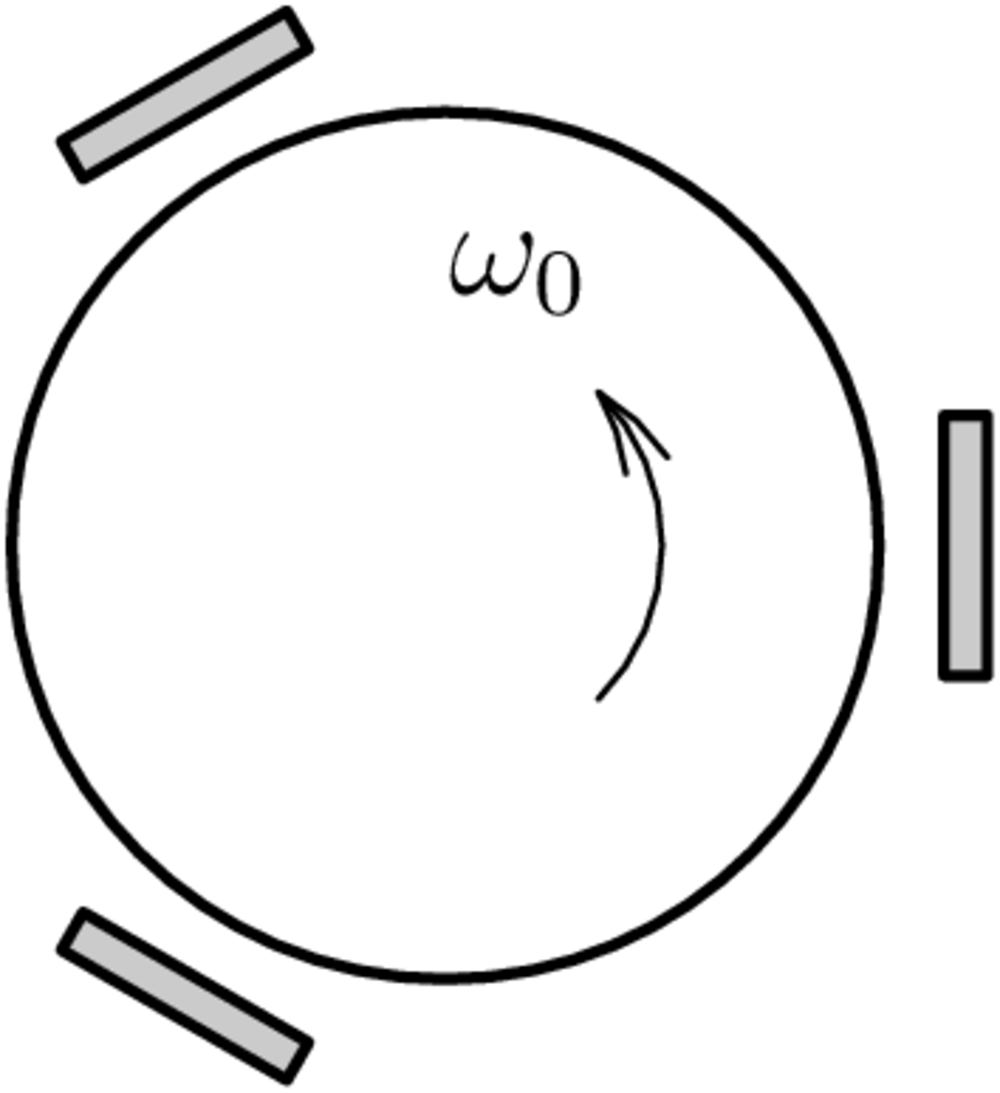
\includegraphics[width=0.8\textwidth]{content/pic/asypng/pic_nu_self_rot.png}
                    % \asyinclude{content/pic/asy/pic_nu_self_rot.asy}
                    \caption{Движение \huge{$1$}}
                \endminipage
                \quad
                \minipage{0.3\textwidth}
                    \hspace{60pt}
                    \centering
                    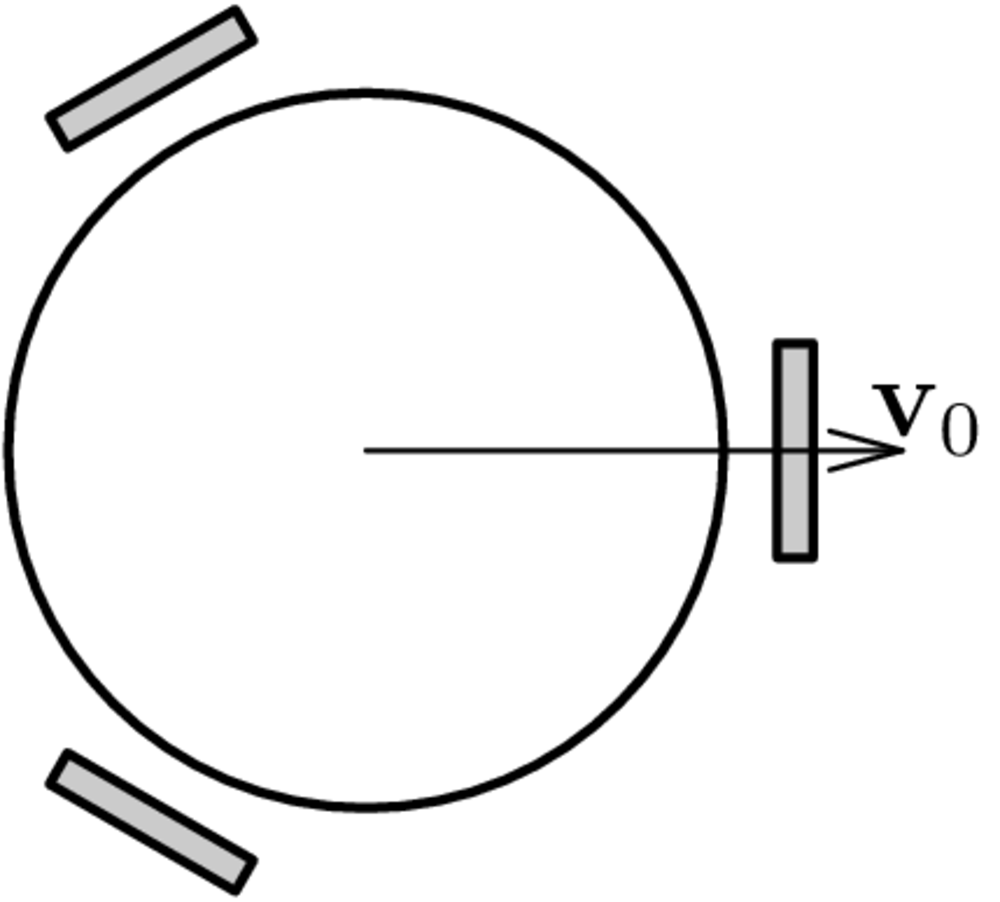
\includegraphics[width=\textwidth]{content/pic/asypng/pic_nu_straight.png}
                    % \asyinclude{content/pic/asy/pic_nu_straight.asy}
                    \caption{Движение \huge{$2$}}
                \endminipage
                \quad
                \minipage{0.3\textwidth}
                    \hspace{60pt}
                    \centering
                    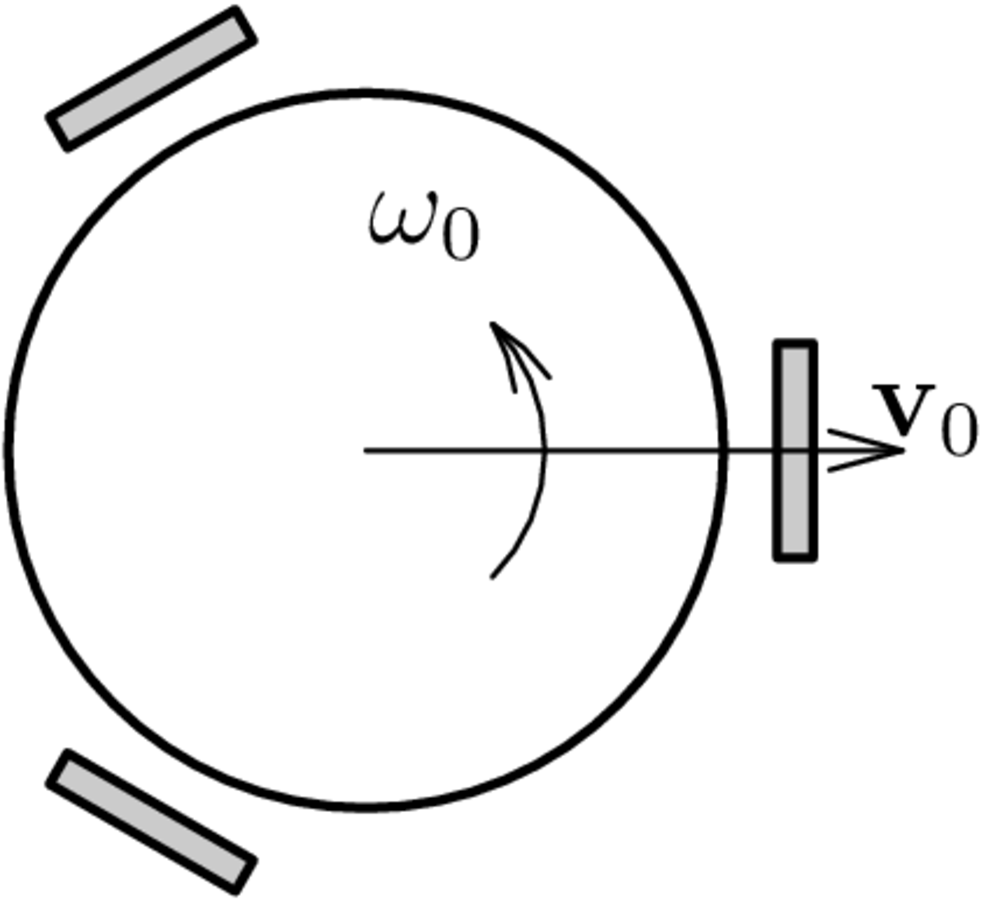
\includegraphics[width=\textwidth]{content/pic/asypng/pic_nu_wrench.png}
                    % \asyinclude{content/pic/asy/pic_nu_wrench.asy}
                    \caption{Движение \huge{$3$}}
                \endminipage
            \end{figure}
            \vspace{10pt}
        }
    }
    
\end{myposter}
